\chapter[Agent Based Simulation]{Agent Based Simulation}

\chapterinitial{S}{ometimes} individual behaviours and
interactions are well understood,
and an understanding of how a whole population of such
individuals might behave needed. For example psychologists and economists may know a
lot about how individual spenders and vendors behave in response to given
stimuli, but an understanding of how these stimuli might effect the
macro-economy is necessary.
Agent based simulation is a paradigm of
thinking that allows such emergent population level behaviour to be investigated
from individual rules and interactions.

\section{Problem}\label{sec:problem}

Consider a city populated by two categories of household, for example a household
might be fans of Cardiff City FC or Swansea City AFC.  % TODO Maybe include a footnote reference to the FA?
Each household has a
preference for living close to households of the same kind, and will move
around the city while their preferences are not satisfied.
How will these individual preferences affect the overall distribution of fans in
the city?

\section{Theory}\label{sec:theory}

The problem considered here is considered a `classic' one for the paradigm of
agent based simulation, and is usually called Schelling's segregation model.
It features in Thomas Schelling's book `Micromotives and Macrobehaviours', whose % TODO Add footnote reference
title neatly summarises the world view of agent based modelling: we know,
understand, determine, or can control individual micromotives; and from this
we'd like to observe and understand macrobehaviours.

In general an agent based model consists of two components, agents, and an
environment:

\begin{itemize}
  \item Agents are autonomous entities that will periodically choose to take one
        of a number of actions (including the option not to take an action).
        These are chosen in order to maximise that agent's own given utility
        function;
  \item An environment contains a number of agents and defines how their
        interactions affect each other.
        The agents may be homogeneous or heterogeneous, and the
        relationships may change over time, possibly due to the actions taken
        by the agents.
\end{itemize}

In general, an agent will first observe a subset of its environment, for
example it will consider some information about the agents it is currently
close to.
Then it will update some information about itself based on these observations.
This could be recording relevant information from the observations, but could
also include some learning, maybe considering its own previous
actions.
It will then decide on an action to take, and carry out this action. This
decision may be deterministic or random and/or based on its own
attributes from some learning process; with the ultimate aim of
maximising its own utility. In practice, a utility can be represented by a
function that maps the environment to some numeric value.
This process happens to all agents in the environment, possibly simultaneously.
This is summarised in Figure~\ref{fig:abm_diagram}

\begin{figure}
    \begin{center}
        \includestandalone[width=\textwidth]{./assets/abm-diagram}
    \end{center}
    \caption{Representation of an agent interacting with its environment.}
    \label{fig:abm_diagram}
\end{figure}

For the football team supporters problem, each household is an agent.
The environment is the city.
Each household's utility function is to satisfy their preference of living next
to at least a given number of households supporting the same team as them.
Their choices of action are to move house or not to move house.

As a simplification the city will be modelled as a \(50 \times 50\) grid.
Each cell of the grid is a house that can either contain a household of Cardiff
City FC supporters, or contain a household of Swansea City AFC supporters.
A house's neighbours are assumed to be the houses adjacent to it, horizontally,
vertically, and diagonally.
For mathematical simplicity, it is also assumed that the grid is a torus, % TODO Maybe a footnote reference here?
where
houses in the top row are vertically adjacent to the bottom row, and houses in
the rightmost column are horizontally adjacent to the leftmost column.

Every household has a preference \(p\).
This corresponds to the minimum proportion of neighbours they are happy to live
Figure~\ref{fig:schelling_happyunhappy} shows a household of Cardiff City FC
supporters that are happy with their neighbours, and not happy with their
neighbours, when \(p=0.5\). Households supporting Cardiff City FC are shaded
grey.

\begin{figure}
    \begin{center}
        \subfigure[A happy household, with 6 similar neighbours (\(\frac{6}{8} > p = 0.5\))]{\includestandalone[width=0.4\textwidth]{./assets/schelling_happy}}
        \subfigure[An unhappy household, with 2 similar neighbours (\(\frac{2}{8} < p = 0.5\))]{\includestandalone[width=0.4\textwidth]{./assets/schelling_unhappy}}
    \end{center}
    \caption{Example of a household happy and unhappy with its neighbours, when
    \(p=0.5\). Households supporting Cardiff City FC are shaded grey, households
    supporting Swansea City AFC are white.}
    \label{fig:schelling_happyunhappy}
\end{figure}

The original problem stated that households move around the city
whenever they are unhappy with their neighbours.
This long process of selling, searching for, and buying houses can be simplified
to randomly pairing two unhappy households and swapping their houses.
In fact, this can be simplified to consider the houses themselves as agents,
who swap households with each other.

Therefore the model logic is:

\begin{enumerate}
  \item Initialise the model: fill each house in the grid with either a
  household of Cardiff City FC or Swansea City AFC supporters with
  probability \(0.5\) each.
  \item At each discrete time step, for every house:
  \begin{enumerate}
    \item Consider their household's neighbours (\textit{observe}).
    \item Determine if the household is happy (\textit{update}).
    \item If unhappy (\textit{decide}), swap household with another randomly
    chosen house with an unhappy household (\textit{action}).
  \end{enumerate}
\end{enumerate}

After a number of time steps the overall structure of the city can be observed
from this agent based model, as it only explicitly defines individual behaviours
and interactions.  Any population level behaviour that may have emerged without
explicit definition.

\section{Solving with Python}\label{sec:solving-with-python}

Agent based modelling lends itself well to a programming paradigm called
object-orientated programming.
This paradigm lets a number of \textit{objects} from a set of instructions
called a \textit{class} to be built.
These objects can both store information (in Python these are called
\textit{attributes}), and do things (in Python these are called
\textit{methods}).
Object-orientated programming allow for the creation of new classes which can be
used to implement the individual behaviours of an agent based model.

For this problem two classes will be built: a
\mintinline{python}{House} and a \mintinline{python}{City} for them to live in.

The following libraries will be used:

\begin{pyin}
import random
import itertools
import numpy as np
\end{pyin}

Now to define the \mintinline{python}{City}:

\begin{pyin}
class City:
    def __init__(self, size, threshold):
        """Initialises the City object.

        Args:
            size: an integer number of rows and columns
            threshold: a number between 0 and 1 representing
              the minimum acceptable proportion of similar
              neighbours
        """
        self.size = size
        sides = range(size)
        self.coords = itertools.product(sides, sides)
        self.houses = {
            (x, y): House(x, y, threshold, self)
            for x, y in self.coords
        }

    def run(self, n_steps):
        """Runs the simulation of a number of time steps.

        Args:
            n_steps: an integer number of steps
        """
        for turn in range(n_steps):
            self.take_turn()

    def take_turn(self):
        """Swaps all sad households."""
        sad = [h for h in self.houses.values() if h.sad()]
        random.shuffle(sad)
        i = 0
        while i <= len(sad) / 2:
            sad[i].swap(sad[-i])
            i += 1

    def mean_satisfaction(self):
        """Finds the average household satisfaction.

        Returns:
            The average city's household satisfaction
        """
        return np.mean(
            [h.satisfaction() for h in self.houses.values()]
        )
\end{pyin}

This defines a class, a template or a set of instructions that can be used to
create instances of it, called objects.
For the considered problem only one instance of the \mintinline{python}{City}
class will be needed.
However, it is useful to be able to produce more in order to run multiple trials
with different random seeds.
This class contains four methods: \mintinline{python}{__init__},
\mintinline{python}{run}, \mintinline{python}{take_turn} and
\mintinline{python}{mean_satisfaction}.

The \mintinline{python}{__init__} method is run whenever the object is first
created, and initialises the object.
In this case it sets a number of attributes.

\begin{itemize}
     \item First the square grid's \mintinline{python}{size} is defined, which
           is the number of rows and columns of houses it contains.
     \item Next the \mintinline{python}{coords} are defined, a list of tuples
           representing all the possible coordinates of the grid, this uses the
           \mintinline{python}{itertools} library for efficient iteration.
     \item Finally \mintinline{python}{houses} is defined, a dictionary with
           grid coordinates as keys, and instances of the
           \mintinline{python}{House} class.
\end{itemize}


The \mintinline{python}{run} method runs the simulation. For each
\mintinline{python}{n_steps} number of discrete time steps, the city runs the
method \mintinline{python}{take_turn}.
In this method, we first create a list of all the houses with households that
are unhappy with their neighbours; these are put in a random order using the
\mintinline{python}{random} library; and then working inwards from the boundary
houses with sad households are paired up and swap households.

The last method defined here is the \mintinline{python}{mean_satisfaction}
method, which is only used to observe any emergent behaviour.
This calculates the average satisfaction of all the houses in the grid, using
the \mintinline{python}{numpy} library for convenience.

In order to be able to create an instance of the above class, we need to define
a \mintinline{python}{House} class:

\begin{pyin}
class House:
    def __init__(self, x, y, threshold, city):
        """Initialises the House object.

        Args:
            x: the integer x-coordinate
            y: the integer y-coordinate
            threshold: a number between 0 and 1 representing
              the minimum acceptable proportion of similar
              neighbours
            city: an instance of the City class
        """
        self.x = x
        self.y = y
        self.threshold = threshold
        self.kind = random.choice(["Cardiff", "Swansea"])
        self.city = city

    def satisfaction(self):
        """Determines the household's satisfaction level.

        Returns:
            A proportion
        """
        same = 0
        for x, y in itertools.product([-1, 0, 1], [-1, 0, 1]):
            ax = (self.x + x) % self.city.size
            ay = (self.y + y) % self.city.size
            same += self.city.houses[ax, ay].kind == self.kind
        return (same - 1) / 8

    def sad(self):
        """Determines if the household is sad.

        Returns:
            a Boolean
        """
        return self.satisfaction() < self.threshold

    def swap(self, house):
        """Swaps two households.

        Args:
            house: the house object to swap household with
        """
        self.kind, house.kind = house.kind, self.kind
\end{pyin}

It contains four methods: \mintinline{python}{__init__},
\mintinline{python}{satisfaction}, \mintinline{python}{sad} and
\mintinline{python}{swap}.

The \mintinline{python}{__init__} methods sets a number of attributes at the
time the object is created: the house's \mintinline{python}{x} and
\mintinline{python}{y} coordinates (its column and row numbers on the grid);
its \mintinline{python}{threshold} which corresponds to \(p\); its
\mintinline{python}{kind} which is randomly chosen between having a Cardiff City
FC supporting household or a Swansea City AFC supporting household; and finally
its \mintinline{python}{city}, an instance of the \mintinline{python}{City}
class, shared by all the houses.

The \mintinline{python}{satisfaction} method loops though each of the house's
neighbouring cells in the city grid, counts the number of neighbours that are
of the same kind as itself, and returns this as a proportion.
Then the \mintinline{python}{sad} method returns a boolean indicating if the
household's satisfaction is below the minimum threshold.

Finally the \mintinline{python}{swap} method takes another house object, and
swaps their household kinds.

A function to create and run one of these simulations will now be written
with a given random seed, threshold, and number of steps. This function returns
the resulting mean happiness:

\begin{pyin}
def find_mean_happiness(seed, size, threshold, n_steps):
    """Create and run an instance of the simulation.

    Args:
        seed: the random seed to use
        size: an integer number of rows and columns
        threshold: a number between 0 and 1 representing
            the minimum acceptable proportion of similar
            neighbours
        n_steps: an integer number of steps

    Returns:
        The average city's household satisfaction after
        n_steps
    """
    random.seed(seed)
    C = City(size, threshold)
    C.run(n_steps)
    return C.mean_satisfaction()
\end{pyin}

Now consider each household with a threshold of
0.65, and compare the mean happiness after 0 steps and 100 steps.
First 0 steps:

\begin{pyin}
print(find_mean_happiness(0, 50, 0.65, 0))
\end{pyin}

\begin{pyout}
0.4998
\end{pyout}

This is well below the minimum threshold of \(0.65\), and so on average most
households are unhappy.
After 100 steps:

\begin{pyin}
print(find_mean_happiness(0, 50, 0.65, 100))
\end{pyin}

\begin{pyout}
0.9078
\end{pyout}

After 100 time steps the average satisfaction level is much higher.
In fact, it is much higher than each individual household's threshold.
Now consider that this satisfaction level is really a level of how similar
each households' neighbours are, it is actually a level of segregation.
This was the central premise of Schelling's original model, % TODO Repeat the footnote reference?
that overall
emergent segregation levels are much higher than any individuals' personal
preference for segregation.

More analysis methods can be added, including plotting functions.
Figure~\ref{fig:schelling_python_plot} shows the grid at the beginning, after 20
time steps, and after 100 time steps, with households supporting Cardiff City FC
in grey, and those supporting Swansea City AFC in white.
It visually shows the households segregating over time.

\begin{figure}
\begin{center}
\subfigure[At the beginning.]{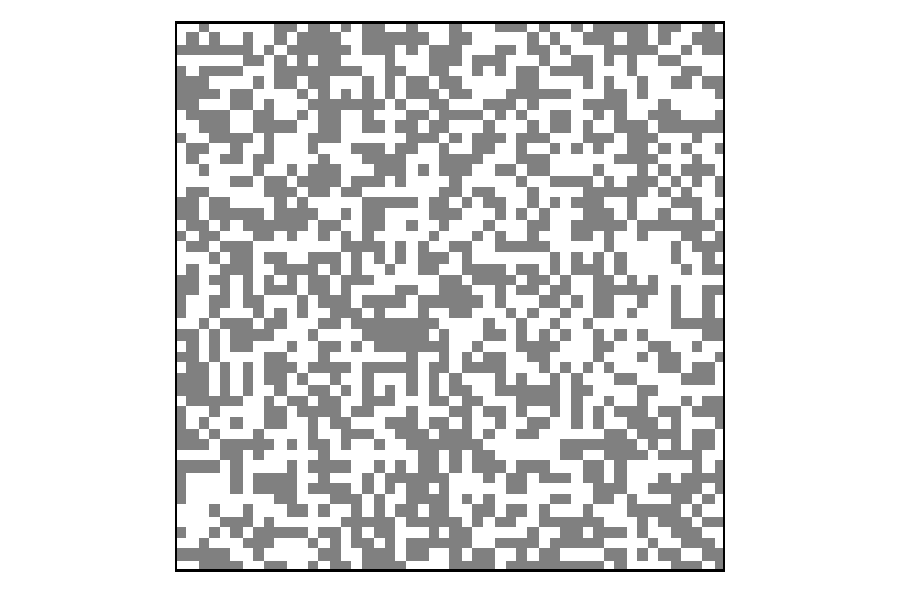
\includegraphics[width=0.32\textwidth]{./assets/python_schelling_0}}
\subfigure[After 20 time steps.]{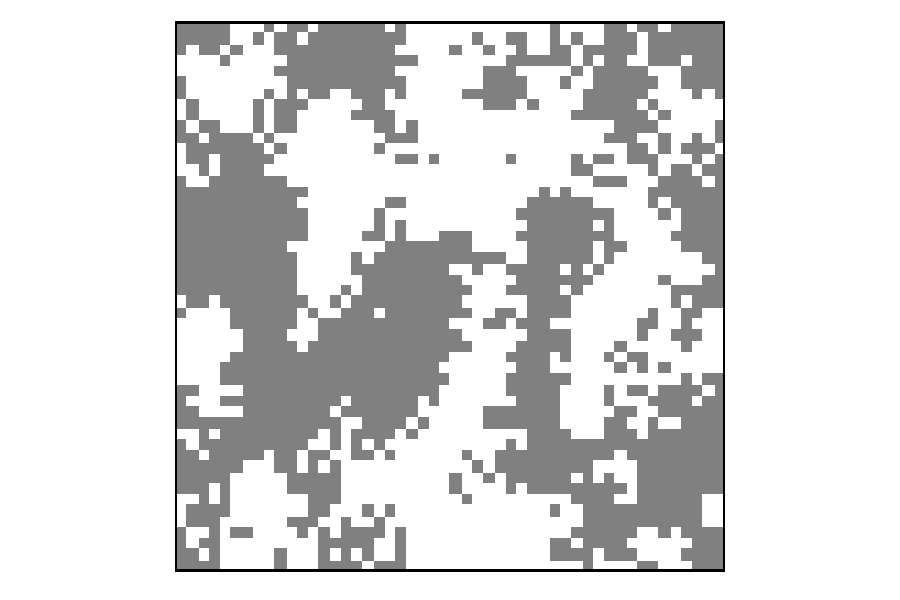
\includegraphics[width=0.32\textwidth]{./assets/python_schelling_20}}
\subfigure[After 100 time steps.]{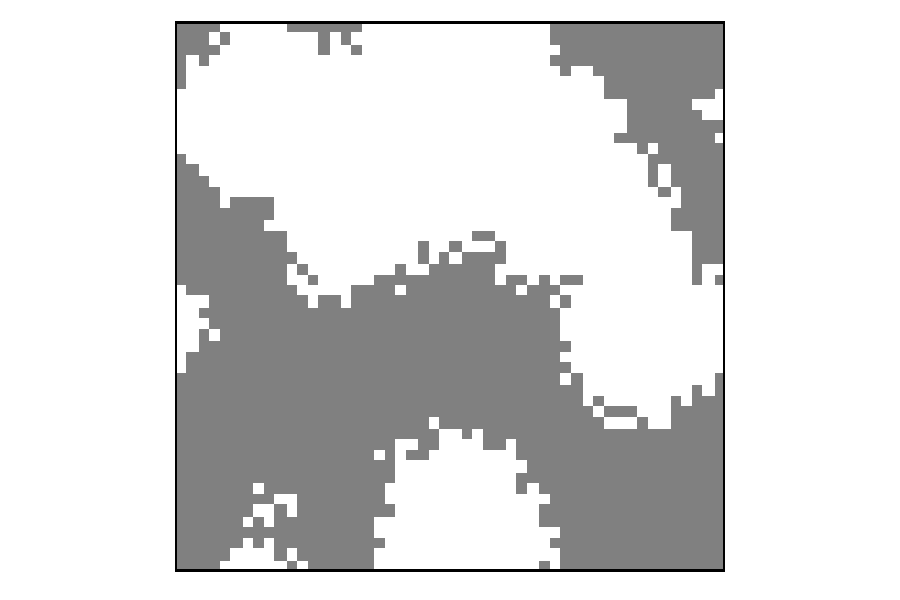
\includegraphics[width=0.32\textwidth]{./assets/python_schelling_100}}
\end{center}
\caption{Plotted results from the Python code.}
\label{fig:schelling_python_plot}
\end{figure}

\section{Solving with R}\label{sec:solving-with-R}

Agent based modelling lends itself well to a programming paradigm called
object-orientated programming.
This paradigm lets a number of \textit{objects} from a set of instructions
called a \textit{class} to be built.
These objects can both store information (in the R library used here these are called
\textit{fields}), and do things (in the R library used here these are called
\textit{methods}).
Object-orientated programming allow for the creation of new classes which can be
used to implement the individual behaviours of an agent based model.

There are a number of ways of doing object-orientated programming in R.
In this chapter, a package called \mintinline{R}{R6} will be used here.

For this problem two classes will be built: a
\mintinline{R}{House} and a \mintinline{R}{City} for them to live in.

Now to define the \mintinline{R}{City}: % TODO Add a footnote with something
                                        % like: Note that for the purposes of
% pagination of this book no documentation is included in the definition of the
% class however. 

\begin{Rin}
library(R6)
city <- R6Class("City", list(
  size = NA,
  houses = NA,
  initialize = function(size, threshold) {
    self$size <- size
    self$houses <- c()
    for (x in 1:size) {
      row <- c()
      for (y in 1:size) {
        row <- c(row, house$new(x, y, threshold, self))
      }
      self$houses <- rbind(self$houses, row)
    } },
  run = function(n_steps) {
    if (n_steps > 0) {
      for (turn in 1:n_steps) {
        self$take_turn()
    } } },
  take_turn = function() {
    sad <- c()
    for (house in self$houses) {
      if (house$sad()) {
        sad <- c(sad, house)
      } }
    sad <- sample(sad)
    num_sad <- length(sad)
    i <- 1
    while (i <= num_sad / 2) {
      sad[[i]]$swap(sad[[num_sad - i]])
      i <- i + 1
    } },
  mean_satisfaction = function() {
    mean(sapply(self$houses, function(x) x$satisfaction()))
  })
)
\end{Rin}

This defines an R6 class, a template or a set of instructions that can be used
to create instances of it, called objects.
For our model we only need one instance of the \mintinline{R}{City} class,
although it may be useful to be able to produce more in order to run multiple
trials with different random seeds.
This class contains four methods: \mintinline{R}{initialize},
\mintinline{R}{run}, \mintinline{R}{take_turn} and
\mintinline{R}{mean_satisfaction}.

The \mintinline{R}{initialize} method is run at the time the object is first
created.
It initialises the object by setting a number of its fields:

\begin{itemize}
     \item First the square grid's \mintinline{R}{size} is defined, which
           is the number of rows and columns of houses it contains.
     \item Then the \mintinline{R}{houses} are defined by iteratively repeating
           the \mintinline{R}{rbind} function to create a two-dimensional vector
           of instances of the, yet to be defined, \mintinline{R}{House} class,
           representing the houses themselves.
\end{itemize}

The \mintinline{R}{run} method runs the simulation. For each discrete time
step from 1 to \mintinline{R}{n_steps}, the world runs the method
\mintinline{R}{take_turn}.
In this method, a list of all the houses with households that
are unhappy with their neighbours is created;
these are put in a random order and then working inwards from the boundary,
houses with sad households are paired up and swap households.

The last method defined here is the \mintinline{R}{mean_satisfaction}
method, which is used to observe the emergent behaviour.
This calculates the average satisfaction of all the houses in the grid.

In order to be able to create an instance of the above class,
a \mintinline{R}{House} class is needed:

\begin{Rin}
house <- R6Class("House", list(
  x = NA,
  y = NA,
  threshold = NA,
  city = NA,
  kind = NA,
  initialize = function(x = NA,
                        y = NA,
                        threshold = NA,
                        city = NA) {
    self$x <- x
    self$y <- y
    self$threshold <- threshold
    self$city <- city
    self$kind <- sample(c("Cardiff", "Swansea"), 1)
  },
  satisfaction = function() {
    same <- 0
    for (x in -1:1) {
      for (y in -1:1) {
        ax <- ( (self$x + x - 1) %% self$city$size) + 1
        ay <- ( (self$y + y - 1) %% self$city$size) + 1
        if (self$city$houses[[ax, ay]]$kind == self$kind) {
          same <- same + 1
        } } }
    (same - 1) / 8
  },
  sad = function() {
    self$satisfaction() < self$threshold
  },
  swap = function(house) {
    old <- self$kind
    self$kind <- house$kind
    house$kind <- old
  })
)
\end{Rin}

It contains four methods: \mintinline{R}{initialize},
\mintinline{R}{satisfaction}, \mintinline{R}{sad} and \mintinline{R}{swap}.

The \mintinline{R}{initialize} methods sets a number of the class' fields when
the object is created: the house's \mintinline{R}{x} and \mintinline{R}{y}
coordinates (its column and row numbers on the grid); its
\mintinline{R}{threshold} which corresponds to \(p\); its \mintinline{R}{kind}
which is randomly chosen between having a Cardiff City
FC supporting household or a Swansea City AFC supporting household; and finally
its \mintinline{R}{city}, an instance of the \mintinline{R}{City} class, shared
by all the houses.

The \mintinline{R}{satisfaction} method loops though each of the house's
neighbouring cells in the city grid, counts the number of neighbours that are of
the same kind as itself, and returns this as a proportion.
The \mintinline{R}{sad} method returns a boolean indicating of the
household's satisfaction is below its minimum threshold.

Finally the \mintinline{R}{swap} method takes another house object, and
swaps their household kinds.

A function to create and run one of these simulations will now be written
with a given random seed, threshold, and number of steps. This function return
the resulting mean happiness:

\begin{Rin}
#' Create and run an instance of the simulation.
#'
#' @param seed: the random seed to use
#' @param size: an integer number of rows and columns
#' @param threshold: a number between 0 and 1 representing
#'   the minimum acceptable proportion of similar neighbours
#' @param n_steps: an integer number of steps
#'
#' @return The average city's household satisfaction
#'   after n_steps
find_mean_happiness <- function(seed, size,
                                threshold, n_steps){
  set.seed(seed)
  our_city <- city$new(size, threshold)
  our_city$run(n_steps)
  our_city$mean_satisfaction()
}
\end{Rin}


Now consider each household with a threshold of
0.65, and compare the mean happiness after 0 steps and 100 steps.
First 0 steps:

\begin{Rin}
print(find_mean_happiness(0, 50, 0.65, 0))
\end{Rin}

\begin{Rout}
[1] 0.4956
\end{Rout}

This is well below the minimum threshold of \(0.65\), and so on average most
households are unhappy here.
Let's run the simulation for 100 generations and see how this changes:

\begin{Rin}
print(find_mean_happiness(0, 50, 0.65, 100))
\end{Rin}

\begin{Rout}
[1] 0.9338
\end{Rout}

After 100 time steps the average satisfaction has increased.
It is now actually much higher that each individual household's threshold.
We can consider this satisfaction level as a level of how similar each
households' neighbours are, and so it is actually a level of segregation.
This was the central premise of Schelling's original model, that overall  % TODO Repeat the footnote reference
emergent segregation levels are much higher than any individuals' personal
preference for segregation.

More analysis methods can be added, including plotting functions.
Figure~\ref{fig:schelling_R_plot} shows the grid at the beginning, after 20
time steps, and after 100 time steps, with households supporting Cardiff City FC
in grey, and those supporting Swansea City AFC in white.
It shows the households segregating over time.

\begin{figure}
\begin{center}
\subfigure[At the beginning.]{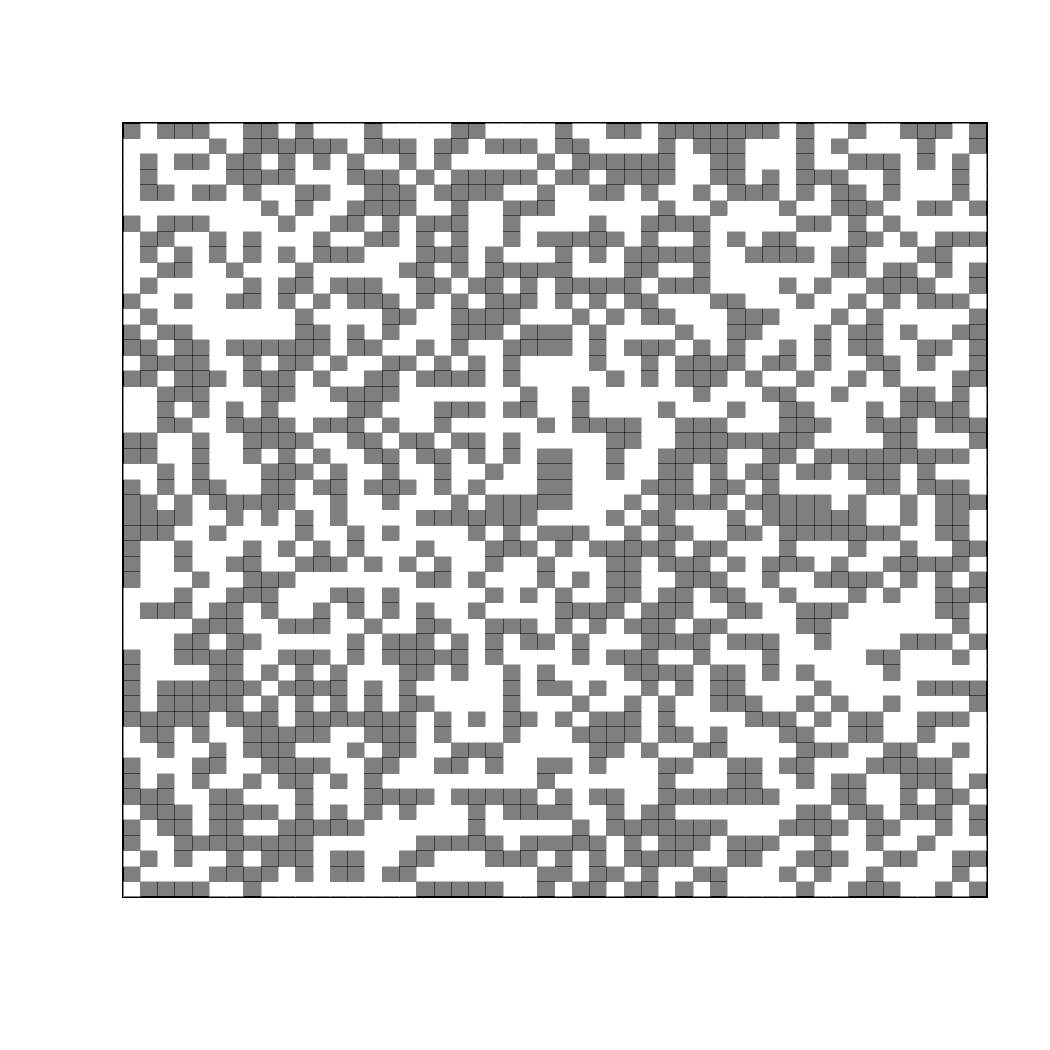
\includegraphics[width=0.32\textwidth]{./assets/schelling_R_0}}
\subfigure[After 20 time steps.]{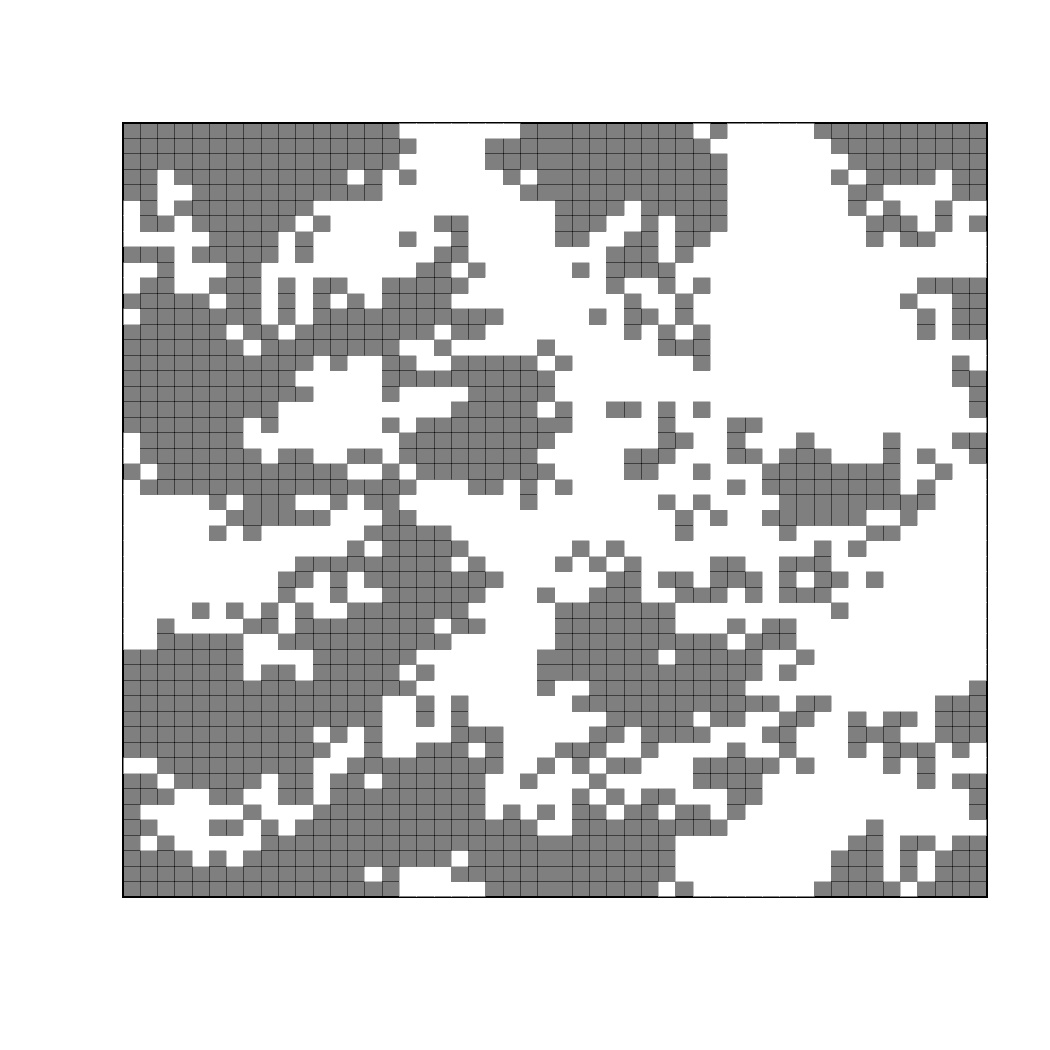
\includegraphics[width=0.32\textwidth]{./assets/schelling_R_20}}
\subfigure[After 100 time steps.]{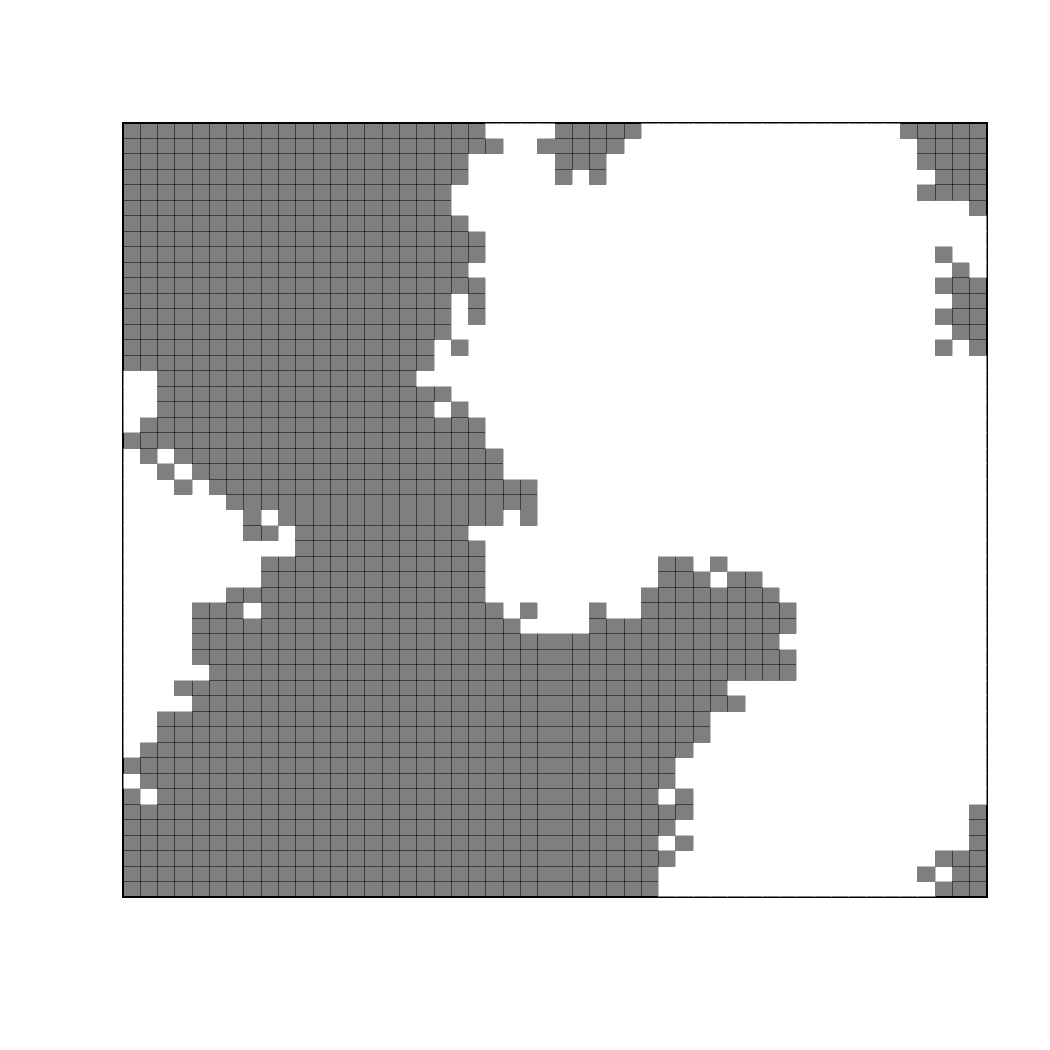
\includegraphics[width=0.32\textwidth]{./assets/schelling_R_100}}
\end{center}
\caption{Plotted results from the R code.}
\label{fig:schelling_R_plot}
\end{figure}

\section{Research}\label{sec:research}

% TODO Even though we will footnote reference it I feel that Schelling's model
% should be here also.
